
%%%
% Things that happened after the experiments
%%%

\subsection{Round 1}

%%%
% Discussion of Round 1:
%	1. graphs to show how strategies were learned
%		4-5 frames to get a flip-book/transition to see things go on 1 strategy
%		2-3 different final strategy pngs
%	2. Performance:
%		worse than random agent in tournament play
%%%

%%%
Round 1 consisted of 32 agents with randomly allocated starting weights
paired off against each other.
%
These two agents played one million games against each other,
each starting with a random score,
learning and reinforcing their weight vectors after each game.
%%%

%%%
The results of the first round's training on a sample agent can be seen
in Figure~\ref{fig:r1_flip}.
%
Each individual square within the image represents the strength of a single
strategy,
in this case \texttt{hand\_max\_avg},
where white means completely absent and black means completely dominant.
%
Each image was taken at an intermediate stage to capture and show transitions.
%%%

%%%
%%%

% Figure for the flipbook of strategies over time

\begin{figure}
\center

	\begin{subfigure}[t]{0.3\textwidth}
	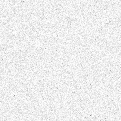
\includegraphics[width=\textwidth]{images/findings/round1/flipbook_a.png}
	\caption{Starting Weights}
	\end{subfigure}
	~
	\begin{subfigure}[t]{0.3\textwidth}
	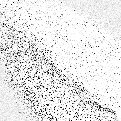
\includegraphics[width=\textwidth]{images/findings/round1/flipbook_b.png}
	\caption{After 200,000 games played}
	\end{subfigure}
	~
	\begin{subfigure}[t]{0.3\textwidth}
	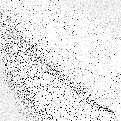
\includegraphics[width=\textwidth]{images/findings/round1/flipbook_c.png}
	\caption{After 400,000 games played}
	\end{subfigure}

	\begin{subfigure}[t]{0.3\textwidth}
	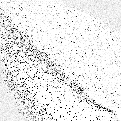
\includegraphics[width=\textwidth]{images/findings/round1/flipbook_d.png}
	\caption{After 600,000 games played}
	\end{subfigure}
	~
	\begin{subfigure}[t]{0.3\textwidth}
	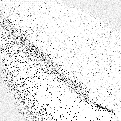
\includegraphics[width=\textwidth]{images/findings/round1/flipbook_e.png}
	\caption{After 800,000 games played}
	\end{subfigure}
	~
	\begin{subfigure}[t]{0.3\textwidth}
	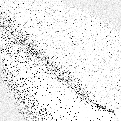
\includegraphics[width=\textwidth]{images/findings/round1/flipbook_f.png}
	\caption{Final Weights}
	\end{subfigure}

\caption{%
	Training weights representation for Agent 0's \handmaxavg\
	strategy when the agent is the dealer
	over the course of the one million games of Round 1.
	In these images, the y-axis represents the player's own score,
	the x-axis the opponent's score,
	with the origin starting at the top-left of the image.
	% N.B. This is correct of generated images from the python code
	%	as of 2018-03-08 19:12.
	% no later modifications will be made from the python code directly to
	% save myself the headache. maybe this will be converted later to be
	% more easily human understood
	% Rotate 90 deg counter-clockwise will make x=my_score, y=opp_score
}
% TODO: figure out axes
% TODO: change these images to hand_max_min: much starker contrast
\label{fig_r1-flip}
\end{figure}

